\section{OAuth}
\label{oautheinleitung}
Wenn ein Benutzer einer Anwendung den Zugriff auf seine Daten erlauben möchte, die von einer weiteren Anwendung verwaltet wird, so kann er Dank des offenen OAuth Protokolls\footnote{\url{http://oauth.net/documentation}}, dieses ohne seine Zugangsdaten preiszugeben.
Dieses Konzept wird besonders bei \acp{API} eingesetzt.
Prominente Beispiele dafür sind Facebook und Twitter.
Diese ermöglichen es, dass Entwickler eigene \acp{App} in das System integrieren können, welche Zugriff auf Benutzerdaten erhalten.
Meldet sich ein Benutzer bei einer Anwendung eines Drittanbieters an, so wird dieser auf die Webseite des eigentlichen Anbieters, also beispielsweise Twitter weitergeleitet, wo er sich anmelden muss.
Twitter schickt dann einen benutzerspezifischen Schlüssel an die Anwendung, mit dem diese dann Zugriff auf die Benutzerdaten erhält.
In vielen \acp{API} wird der Benutzer zusätzlich noch darauf hingewiesen, auf welche Daten die Anwendung Zugriff erhält.
Dies ist jedoch nicht Bestandteil der OAuth Spezifikation.

\subsection{Historischer Hintergrund}
Bevor OAuth entwickelt wurde, arbeiteten bereits einige Firmen, wie beispielsweise Twitter\footnote{\url{http://www.twitter.com}} und Ma.gnolia\footnote{\url{http://gnolia.com}}, an der Implementierung des OpenID\footnote{\url{http://openid.net}} Protokolls in ihren Webanwendungen.
Jedoch war dieses Verfahren nicht für autorisierungspflichtige Schnittstellen ausgelegt, da ein Benutzer, der OpenID verwendet, kein Passwort mehr hat.
Dieses ist allerdings zwingend notwendig, da er sich sonst nicht an der Schnittstelle anmelden kann.
Es existierten bereits einige alternative Verfahren, wie beispielsweise Flickr Auth, Google AuthSub oder Yahoo! BBAuth, jedoch kein definierter Standard.
Daraufhin wurde im Dezember 2006 ein Treffen zwischen diversen Entwicklern und David Recordon, einem Entwickler von OpenID, organisiert, bei dem über einen Authentifizierungsstandard diskutiert werden sollte.
Aus dem Treffen entstand OpenAuth, welche später zu OAuth umbenannt wurde.
Im Oktober 2007 wurde die finale OAuth Core 1.0 Spezifikation veröffentlicht\cite[vgl.][]{oauth11}.

Knapp fünf Jahre später, im Oktober 2012 wurde die OAuth 2.0 Spezifikation herausgebracht\cite[vgl.][]{oauth12}.
An diesem Verfahren gab es jedoch viel auszusetzen, was Eran Hammer\footnote{\url{http://hueniverse.com/author/eran}}, einen Mitbegründer der OAuth 1.0 und OAuth 2.0 Spezifikation, dazu veranlasste, von seinem Posten als Vorsitzender des OAuth Komitees, zurückzutreten\cite[vgl.][]{eran10}.
Er selbst sagt, dass OAuth 2.0 im Vergleich zum OAuth 1.0 "`viel komplexer, weniger interoperabel, weniger nützlich, unvollständiger und vor allem weniger sicher"'\cite{eran12} ist.
Dennoch wird diese Methode in der Praxis verwendet und löst nach und nach OAuth 1.0 ab.

\subsection{OAuth 1.0}
In der Spezifikation von OAuth 1.0 werden drei Rollen festgelegt.
Es gibt den \frqq Consumer\flqq , welcher dem Client oder auch einer Anwendung entspricht, der \frqq Service Provider\flqq , welcher der Server ist, beispielsweise Twitter, und der \frqq User\flqq , der auch als Resource Owner bezeichnet wird\cite[vgl.][]{oauth10}.
In einem klassischen Client-Server Authentifizierungsverfahren muss der User seine Zugangsdaten, welche meist aus einer Email oder einem Benutzernamen und einem Passwort bestehen, beim Server eingeben\cite[vgl.][]{oauth11}.
Dabei ist es dem Server egal, von wem er diese Daten erhält, unabhängig davon, ob es der User selbst ist oder ein anderer Anbieter\cite[vgl.][]{oauth11}.
Sobald ein Drittanbieter an diesem Prozess beteiligt ist, hat dieses Verfahren einen gewaltigen Nachteil.
Der Drittanbieter bekommt Kenntnis über die eigentlich geheimen Zugangsdaten des Users.
Durch die Verwendung von OAuth bleiben diese Zugangsdaten jedoch beim Server und der Client interagiert nur noch mit Hilfe eines Tokens mit dem Server.

Die Anzahl der eingebundenen Anbieter wird durch eine Anzahl von \frqq Füßen\flqq\ beschrieben.
So wäre beispielsweise der letztgenannte Fall eine 3-beinige Authentifizierung, im Englischen 3-legged Authentication genannt.
Weiteres Legs werden unterschiedlich definiert, wobei generell gilt, dass sobald ein Anbieter Zugriff auf die Nutzerdaten beansprucht, dieser als ein weiteres Leg gezählt wird\cite[vgl.][]{oauth11}.

Weiterhin gibt es drei Arten von Token, also einzigartige Schlüssel, in der OAuth Spezifikation.
Diese werden als \frqq client credentials\flqq , \frqq temporary credentials\flqq\ und \frqq token credentials\flqq\ bezeichnet\cite[vgl.][]{oauth11}.
Zu den \frqq client credentials\flqq\ zählt der \frqq consumer key\flqq\ und das \frqq consumer secret\flqq\cite[vgl.][]{oauth11}.
Diese kennt der Consumer und benötigt diese, um dem Service Provider mitzuteilen, welche Anwendung Zugriff auf Benutzerdaten haben möchte.

Der \frqq request token\flqq\ und das \frqq request secret\flqq\ gehören zu den \frqq temporary credentials\flqq , welche der Consumer benutzt, um den Service Provider aufzufordern den User zu verifizieren\cite[vgl.][]{oauth11}.

Als \frqq token credentials\flqq\ werden der \frqq access token\flqq\ und das \frqq access secret\flqq\ bezeichnet\cite[vgl.][]{oauth11}.
Diese dienen nach einer erfolgreichen Authentifizierung fortan als Erkennungsschlüssel für den User.
Ein Consumer kann mit den Token Benutzerdaten anfordern oder diese bearbeiten.

Abbildung \ref{fig-oauth-workflow} zeigt das Verfahren schematisch auf.

\begin{figure}[H]
  \centering
  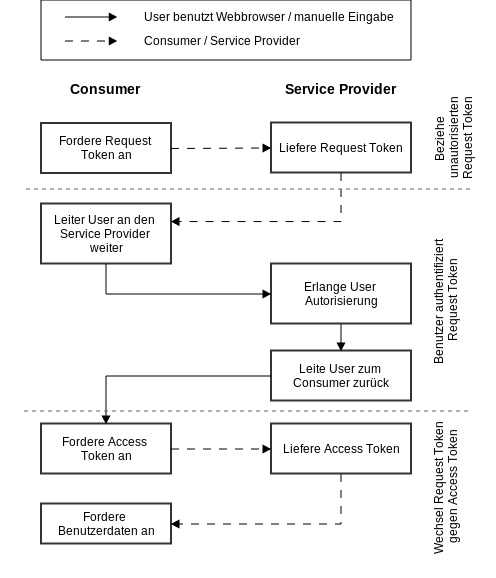
\includegraphics[scale=0.6]{resources/Bilder_Kapitel_2/oauth_workflow.png}
  \caption[Workflow des OAuth 1.0 Authentifizierungsprozesses]{Workflow des OAuth 1.0 Authentifizierungsprozesses (In Anlehnung an \cite{oauthdiagramm07})}
  \label{fig-oauth-workflow}
\end{figure}

In der Praxis würde sich der User beispielsweise für ein Textverarbeitungsprogramm von Google, welcher in diesem Fall der Consumer ist, interessieren.
Die Dateien, die er bearbeiten möchte, liegen jedoch bei Dropbox, dem Service Provider.
Der User möchte nun Google für den Zugriff auf seine Daten bei Dropbox berechtigen.
Dropbox verwendet eine offene \ac{API}, welche OAuth unterstützt und Google hat bereits bei dieser eine Entwickleranwendung angelegt.
Nach dem Anlegen hat Google die \frqq client credentials\flqq\ für seine Anwendung erhalten.

Wenn der User nun Google dazu berechtigen möchte, auf seine Benutzerdaten zugreifen zu können, muss er dazu einen Button auf der Webseite von Google betätigen.
Daraufhin werden zwei Vorgänge durchgeführt.
Zuerst schickt Google seine \frqq client credentials\flqq\ an Dropbox und erhält, insofern diese Gültig sind, die \frqq temporary credentials\flqq\ zurück.
Sobald Google diese erhalten hat, wird der User auf die Loginseite von Dropbox weitergeleitet.
Dort gibt er seine Zugangsdaten ein, um seine Authentizität zu beweisen.
Nachdem er eingeloggt ist, bekommt er eine Bestätigungsseite angezeigt, auf der er Google Zugriff auf seine Daten gewähren kann.
Hat er dem zugestimmt, wird er zu Google zurückgeleitet.
Google erhält daraufhin den \frqq request token\flqq\ zurück, welcher ihm aufzeigt, dass ihm der User den Zugriff gewährt hat.
Abschließend schickt Google seinen \frqq consumer key\flqq\ und den \frqq request token\flqq\ an Dropbox und erhält die \frqq token credentials\flqq .
Mit diesen kann Google fortan die Benutzerdaten von Dropbox abrufen, verändern und die gewünschten Textdateien des Users in seinem Service einbinden.
Im OAuth 1.0 Standard ist jedoch kein Parameter angegeben, welcher den Gültigkeitszeitraum der \frqq token credentials\flqq\ festlegt.
Somit sind diese für immer gültig oder entsprechend der Implementierung des Service Providers werden diese nach einem gewissen Zeitraum verworfen.
Jedoch gibt es keine Vereinheitlichung in diesem Punkt.

\subsection{OAuth 1.0A}
Nachdem im Jahr 2009 eine Sicherheitslücke in der OAuth 1.0 Methode entdeckt wurde, haben Google und Yahoo! eine weitere Revision von OAuth 1.0, welche später als OAuth 1.0A veröffentlicht wurde, entwickelt\cite[vgl.][]{oauth10a}.
Der Angriff auf das Authentifizierungsverfahren, welcher als \frqq session fixation attack\flqq\ bezeichnet wird, hat folgenden Ablauf.

Der Angreifer Mallory möchte ein Textdokument aus seiner Dropbox mit dem Google Textbearbeitungsprogramm bearbeiten.
Er initiiert dazu den OAuth Autorisierungsprozess bei Google, unterbindet jedoch die Weiterleitung zu Dropbox und speichert sich den Link dahin ab.
Dieser enthält die \frqq client credentials\flqq\ und die URL zur Authentifizierungsseite.
Nachfolgend bringt er einen Benutzer Alice dazu, diesen Link anzuklicken.

Alice führt den von Mallory gestarteten Autorisierungsprozess fort und wird zu Dropbox geleitet.
Dort gibt sie ihre Benutzerdaten ein und akzeptiert die Berechtigung der Google \ac{App} Zugriff auf ihre Daten zu haben.
Sie bekommt jedoch nicht mit, dass ein Angriff durchgeführt wird, da sie sich beim gültigen Serviceprovider befindet und auch die korrekte \ac{App} angezeigt bekommt.
Nachdem Alice zurück zur Applikation geleitet wurde, führt Mallory seinen Autorisierungsprozess fort, indem er die Weiterleitung von Dropbox zurück zu Google nachbaut oder diese bei Alice manipuliert.
Von diesem Zeitpunkt an ist der Dropbox-Account von Alice mit der Google \ac{App} von Mallory verbunden.

Das ganze Verfahren ähnelt einem Pishingverfahren und setzt auf Social Engineering, was bedeutet, dass das Vertrauen und die Gewohnheit eines unachtsamen Benutzers ausgenutzt wird und dieser einem Link aus einer nicht vertrauenswürdigen Quelle folgt.

Um diese Sicherheitslücke zu schließen, wurde als vorzeitige Lösung ein Warnhinweis vom Serviceprovider, also im Beispiel Dropbox, angezeigt, wenn der Benutzer von einer \ac{URL} weitergeleitet wurde, die nicht mit der \ac{URL} des \ac{App} Betreibers übereinstimmt, im Beispiel Google\cite[vgl.][]{session-fixation-attack}.
Diese Variante hat sich jedoch als unzureichend herausgestellt, sodass das OAuth 1.0A Protokoll entwickelt wurde.

In OAuth 1.0A wurden drei wesentliche Änderungen durchgeführt.
Wenn der Consumer die \frqq temporary credentials\flqq\ beim Service Provider anfordert, muss er eine Callback URL angeben\cite[vgl.][]{oauth10a}.
Dieser Parameter existierte bereits in der OAuth 1.0 Spezifikation, war dort aber optional und wurde erst beim Weiterleiten zum Service Provider mitgesendet, wenn die \frqq session fixation attack\flqq\ bereits gestartet ist.
Nach Abschluss der Autorisierung beim Service Provider wird der User an diese URL weitergeleitet.

Weiterhin wurde der Parameter \frqq oauth\_callback\_confirmed\flqq\ eingeführt, der den Wert true hat und bei der Anfrage des \frqq request token\flqq\ an den Consumer geschickt wird\cite[vgl.][]{oauth10a}.
Dieser dient lediglich zur Erkennung einer OAuth 1.0A Unterstützung Seitens des Service Providers.

Die letzte Änderung betrifft die Weiterleitung des Users vom Service Provider zum Consumer.
Hierbei wird der Parameter \frqq oauth\_verifier\flqq\ implementiert, der vom Consumer entgegengenommen und bei der Anfrage der \frqq token credentials\flqq\ mitgeschickt werden muss\cite[vgl.][]{oauth10a}.

Diese drei Änderungen haben die \frqq session fixation attack\flqq\ ungültig gemacht.
Das OAuth Komitee hat darüber hinaus jedem Anbieter dringendst geraten sein System auf OAuth 1.0A zu aktualisieren\cite[vgl.][]{session-fixation-attack}.

\subsection{OAuth 2.0}
\label{authentifizierung-oauth-2}
OAuth 2.0 wurde im Oktorber 2012 veröffentlicht und ist ein komplett neues Protokoll, welches nicht abwärtskompatibel zu OAuth 1.0 oder OAuth 1.0A ist\cite[vgl.][]{eran10}.
Es gibt wesentliche Veränderung im Workflow und in der Kommunikation mit dem Server.
Dabei sind drei Unterschiede als besonders prägnant zu erachten.
Jegliche Verbindungen erfolgen über \ac{SSL} und es muss keine eigene Signatur, wie bei den vorherigen OAuth Protokollen, erzeugt und geprüft werden\cite[vgl.][]{oauth12}.

Des Weiteren existiert nur noch ein Token in den \frqq token credentials\flqq .
Dieser wird \frqq access\_token\flqq\ genannt und dient fortan zur Authentifizierung des Users\cite[vgl.][]{oauth12}.
Ein optionaler \frqq refresh\_token\flqq\ kann vom Service Provider an den Consumer geschickt werden, welcher oftmals mit einem Parameter \frqq expires\_in\flqq\ übergeben wird\cite[vgl.][]{oauth12}.
Letzterer gibt in Millisekunden an, wie lange der \frqq access\_token\flqq\ gültig ist\cite[vgl.][]{oauth12}.
Sollte dieser abgelaufen sein, so kann ohne das Eingreifen des Users mithilfe des \frqq refresh\_token\flqq\ ein Neuer angefordert werden.
Ein weiterer Vorteil dieses Prinzips ist, dass die Laufzeit der \frqq token credentials\flqq\ explizit festgelegt wird und diese nicht wie bei OAuth 1.0 einen unbegrenzten Verwendungszeitraum ermöglichen.
Häufig wird dieser Zeitraum auf 3600 Millisekunden, also eine Stunde, festgesetzt.
Das OAuth Komitee empfiehlt dringend die Implementierung des \frqq refresh\_token\flqq\ und des \frqq expires\_in\flqq\ Parameters, jedoch sind beide optional, womit die Entscheidung beim Service Provider liegt, diese zu verwenden oder nicht\cite[vgl.][]{oauth12}.

Weiterhin gibt es vier Rollen im OAuth 2.0 Standard.
Es gibt den \frqq resource owner\flqq , welcher dem User entspricht, also einem Benutzer einer Anwendung\cite[vgl.][]{oauth12}.
Ebenfalls gleich geblieben ist der Client, welcher auch als Consumer bezeichnet wird\cite[vgl.][]{oauth12}.
Neu ist die Unterteilung in einem \frqq resource server\flqq\ und einem \frqq authorization server\flqq\cite[vgl.][]{oauth12}.
Der \frqq resource server\flqq\ hält die Benutzerdaten vor, während der \frqq authorization server\flqq\ die \frqq credentials\flqq , also jegliche Token speichert\cite[vgl.][]{oauth12}.
Diese Unterteilung erleichtert die Implementierung des Protokolls auf Seiten des Server Providers, der meist beide Rollen zugleich einnimmt.
Lediglich die Domain kann voneinander abweichen.

Der Workflow von OAuth 2.0 hat sich in der Praxis wie folgt verändert.
Wie bereits in den vorherigen Spezifikationen muss der Consumer eine Entwicklerapp beim Service Provider anlegen.
Dabei muss er bereits eine Callback \ac{URL} definieren, an die der User nach dem Autorisierungsprozess weitergeleitet wird.
Der Consumer erhält nach Abschluss der Erstellung die \frqq client credentials\flqq , also eine \frqq client\_id\flqq\ , sowie ein \frqq client\_secret\flqq .
Sobald ein User einen Consumer Autorisieren möchte, Zugriff auf seine Daten zu erhalten, wird er wie gewohnt zum Service Provider weitergeleitet.
Jedoch entfällt der bisherige Prozess zum Erzeugen der \frqq temporary credentials\flqq .
Der Consumer schickt lediglich seine \frqq client\_id\flqq\ bei Weiterleiten an den Service Provider, wodurch dieser die entsprechende Entwicklerapp eruieren kann.

Beim Service Provider bekommt der Benutzer, wie zuvor, die Loginseite angezeigt und muss nach erfolgreichem Login der Entwicklerapp den Zugriff gewähren oder diesen ablehnen.
Sobald er zugestimmt hat, wird er an die Callback \ac{URL} des Consumers geleitet, welche bei der Erstellung der Entwicklerapp definiert wurde.
Dabei wird ein Parameter mit der Bezeichnung \frqq code\flqq\ mitgeschickt.
Zum Erzeugen eines \frqq access\_tokens\flqq\ muss dieser, samt der \frqq client\_id\flqq\ an den Service Provider geschickt werden.
Dieser überprüft den \frqq code\flqq\ und schickt den \frqq access\_token\flqq , sowie optional den \frqq refresh\_token\flqq\ und die Lebenszeit des \frqq access\_tokens\flqq\ an den Consumer zurück.
Ein Beispiel für solch eine Antwort ist in Quellcode \ref{fig-oauth-response} zu sehen.

\begin{lstlisting}[label=fig-oauth-response,caption={[Aufbau eines Response vom Service Provider an den Consumer]Aufbau eines Response vom Service Provider an den Consumer\cite{oauth12}}]
HTTP/1.1 200 OK
Content-Type: application/json;charset=UTF-8
Cache-Control: no-store
Pragma: no-cache

{
    "access_token":"2YotnFZFEjr1zCsicMWpAA",
    "token_type":"example",
    "expires_in":3600,
    "refresh_token":"tGzv3JOkF0XG5Qx2TlKWIA",
    "example_parameter":"example_value"
}
\end{lstlisting}

Der Consumer kann nun mit den erhaltenden \frqq access\_token\flqq\ auf die Benutzerdaten zugreifen.
Sollte die Lebenszeit des Tokens abgelaufen sein, muss dieser unter Zuhilfenahme des \frqq refresh\_tokens\flqq\ neu angefordert werden.
Das bedeutet, der Consumer macht einen Request mit dem \frqq refresh\_token\flqq\ und der \frqq client\_id\flqq\ an den Service Provider und dieser schickt, sowohl einen neuen \frqq access\_token\flqq , als auch einen neuen \frqq refesh\_token\flqq\ und ein \frqq expires\_in\flqq\ an die Anwendung zurück.
Dieses Verfahren kann beliebig oft wiederholt werden.
